\documentclass[11pt, a4paper]{article}
\usepackage{pdfpages}
\usepackage{parallel}
\usepackage[T2A]{fontenc}
\usepackage{ucs}
\usepackage[utf8x]{inputenc}
\usepackage[polish,english,russian]{babel}
\usepackage{hyperref}
\usepackage{rotating}
\usepackage[inner=2cm,top=1.8cm,outer=2cm,bottom=2.3cm,nohead]{geometry}
\usepackage{listings}
\usepackage{graphicx}
\usepackage{wrapfig}
\usepackage{longtable}
\usepackage{indentfirst}
\usepackage{array}
\usepackage{tikzsymbols}
\usepackage{soul}
\usepackage[ruled,vlined]{algorithm2e}
%\counterwithout{figure}{section} 

\usepackage{url}
\makeatletter
\g@addto@macro{\UrlBreaks}{\UrlOrds}
\makeatother

\newcolumntype{P}[1]{>{\raggedright\arraybackslash}p{#1}}
\frenchspacing
\usepackage{fixltx2e} %text sub- and superscripts
\usepackage{icomma} % коскі ў матэматычным рэжыме
\PreloadUnicodePage{4}

\newcommand{\longpage}{\enlargethispage{\baselineskip}}
\newcommand{\shortpage}{\enlargethispage{-\baselineskip}}

\def\switchlang#1{\expandafter\csname switchlang#1\endcsname}
\def\switchlangbe{
\let\saverefname=\refname%
\def\refname{Літаратура}%
\def\figurename{Іл.}%
}
\def\switchlangen{
\let\saverefname=\refname%
\def\refname{References}%
\def\figurename{Fig.}%
}
\def\switchlangru{
\let\saverefname=\refname%
\let\savefigurename=\figurename%
\def\refname{Литература}%
\def\figurename{Рис.}%
}

\hyphenation{admi-ni-stra-tive}
\hyphenation{ex-pe-ri-ence}
\hyphenation{fle-xi-bi-li-ty}
\hyphenation{Py-thon}
\hyphenation{ma-the-ma-ti-cal}
\hyphenation{re-ported}
\hyphenation{imp-le-menta-tions}
\hyphenation{pro-vides}
\hyphenation{en-gi-neering}
\hyphenation{com-pa-ti-bi-li-ty}
\hyphenation{im-pos-sible}
\hyphenation{desk-top}
\hyphenation{elec-tro-nic}
\hyphenation{com-pa-ny}
\hyphenation{de-ve-lop-ment}
\hyphenation{de-ve-loping}
\hyphenation{de-ve-lop}
\hyphenation{da-ta-ba-se}
\hyphenation{plat-forms}
\hyphenation{or-ga-ni-za-tion}
\hyphenation{pro-gramming}
\hyphenation{in-stru-ments}
\hyphenation{Li-nux}
\hyphenation{sour-ce}
\hyphenation{en-vi-ron-ment}
\hyphenation{Te-le-pathy}
\hyphenation{Li-nux-ov-ka}
\hyphenation{Open-BSD}
\hyphenation{Free-BSD}
\hyphenation{men-ti-on-ed}
\hyphenation{app-li-ca-tion}

\def\progref!#1!{\texttt{#1}}
\renewcommand{\arraystretch}{2} %Іначай формулы ў матрыцы зліпаюцца з лініямі
\usepackage{array}

\def\interview #1 (#2), #3, #4, #5\par{

\section[#1, #3, #4]{#1 -- #3, #4}
\def\qname{LVEE}
\def\aname{#1}
\def\q ##1\par{{\noindent \bf \qname: ##1 }\par}
\def\a{{\noindent \bf \aname: } \def\qname{L}\def\aname{#2}}
}

\def\interview* #1 (#2), #3, #4, #5\par{

\section*{#1\\{\small\rm #3, #4. #5}}
\ifx\ParallelWhichBox\undefined%
    \addcontentsline{toc}{section}{#1, #3, #4}%
\else%
\ifnum\ParallelWhichBox=0%
    \addcontentsline{toc}{section}{#1, #3, #4}%
\fi\fi%

\def\qname{LVEE}
\def\aname{#1}
\def\q ##1\par{{\noindent \bf \qname: ##1 }\par}
\def\a{{\noindent \bf \aname: } \def\qname{L}\def\aname{#2}}
}

\newcommand{\interviewfooter}[1]{
\vskip 1em
\noindent \textit{#1}
}

\switchlang{en}
\begin{document}

\title{1983 "--- DEC VS10X-EA Mouse}
\date{}
\maketitle
\selectlanguage{english}
The DEC VS10X-EA mouse (fig. \ref{fig:DecVS10XPic}) was released in 1983, and it is heavily based on the Hawley Mouse House \cite{hawley,mouses} by Jack Hawley, co-designer of the Xerox Alto computer mouse and one of the authors 1973 Xerox patent for a two-wheel tilt mouse \cite{pat}. In fact, the DEC VS10X-EA is a modification of the Hawley Mark II X063X Mouse of the same year. Comparison of the two mice reveals no techincal differences except the shape of the case and connector. The mouse was supplied with the DEC VAXstation 100 graphical terminals \cite{reddit} used in creation of the X Windows System, a graphical windowing system for Unix-like OS.

\begin{figure}[h]
   \centering
    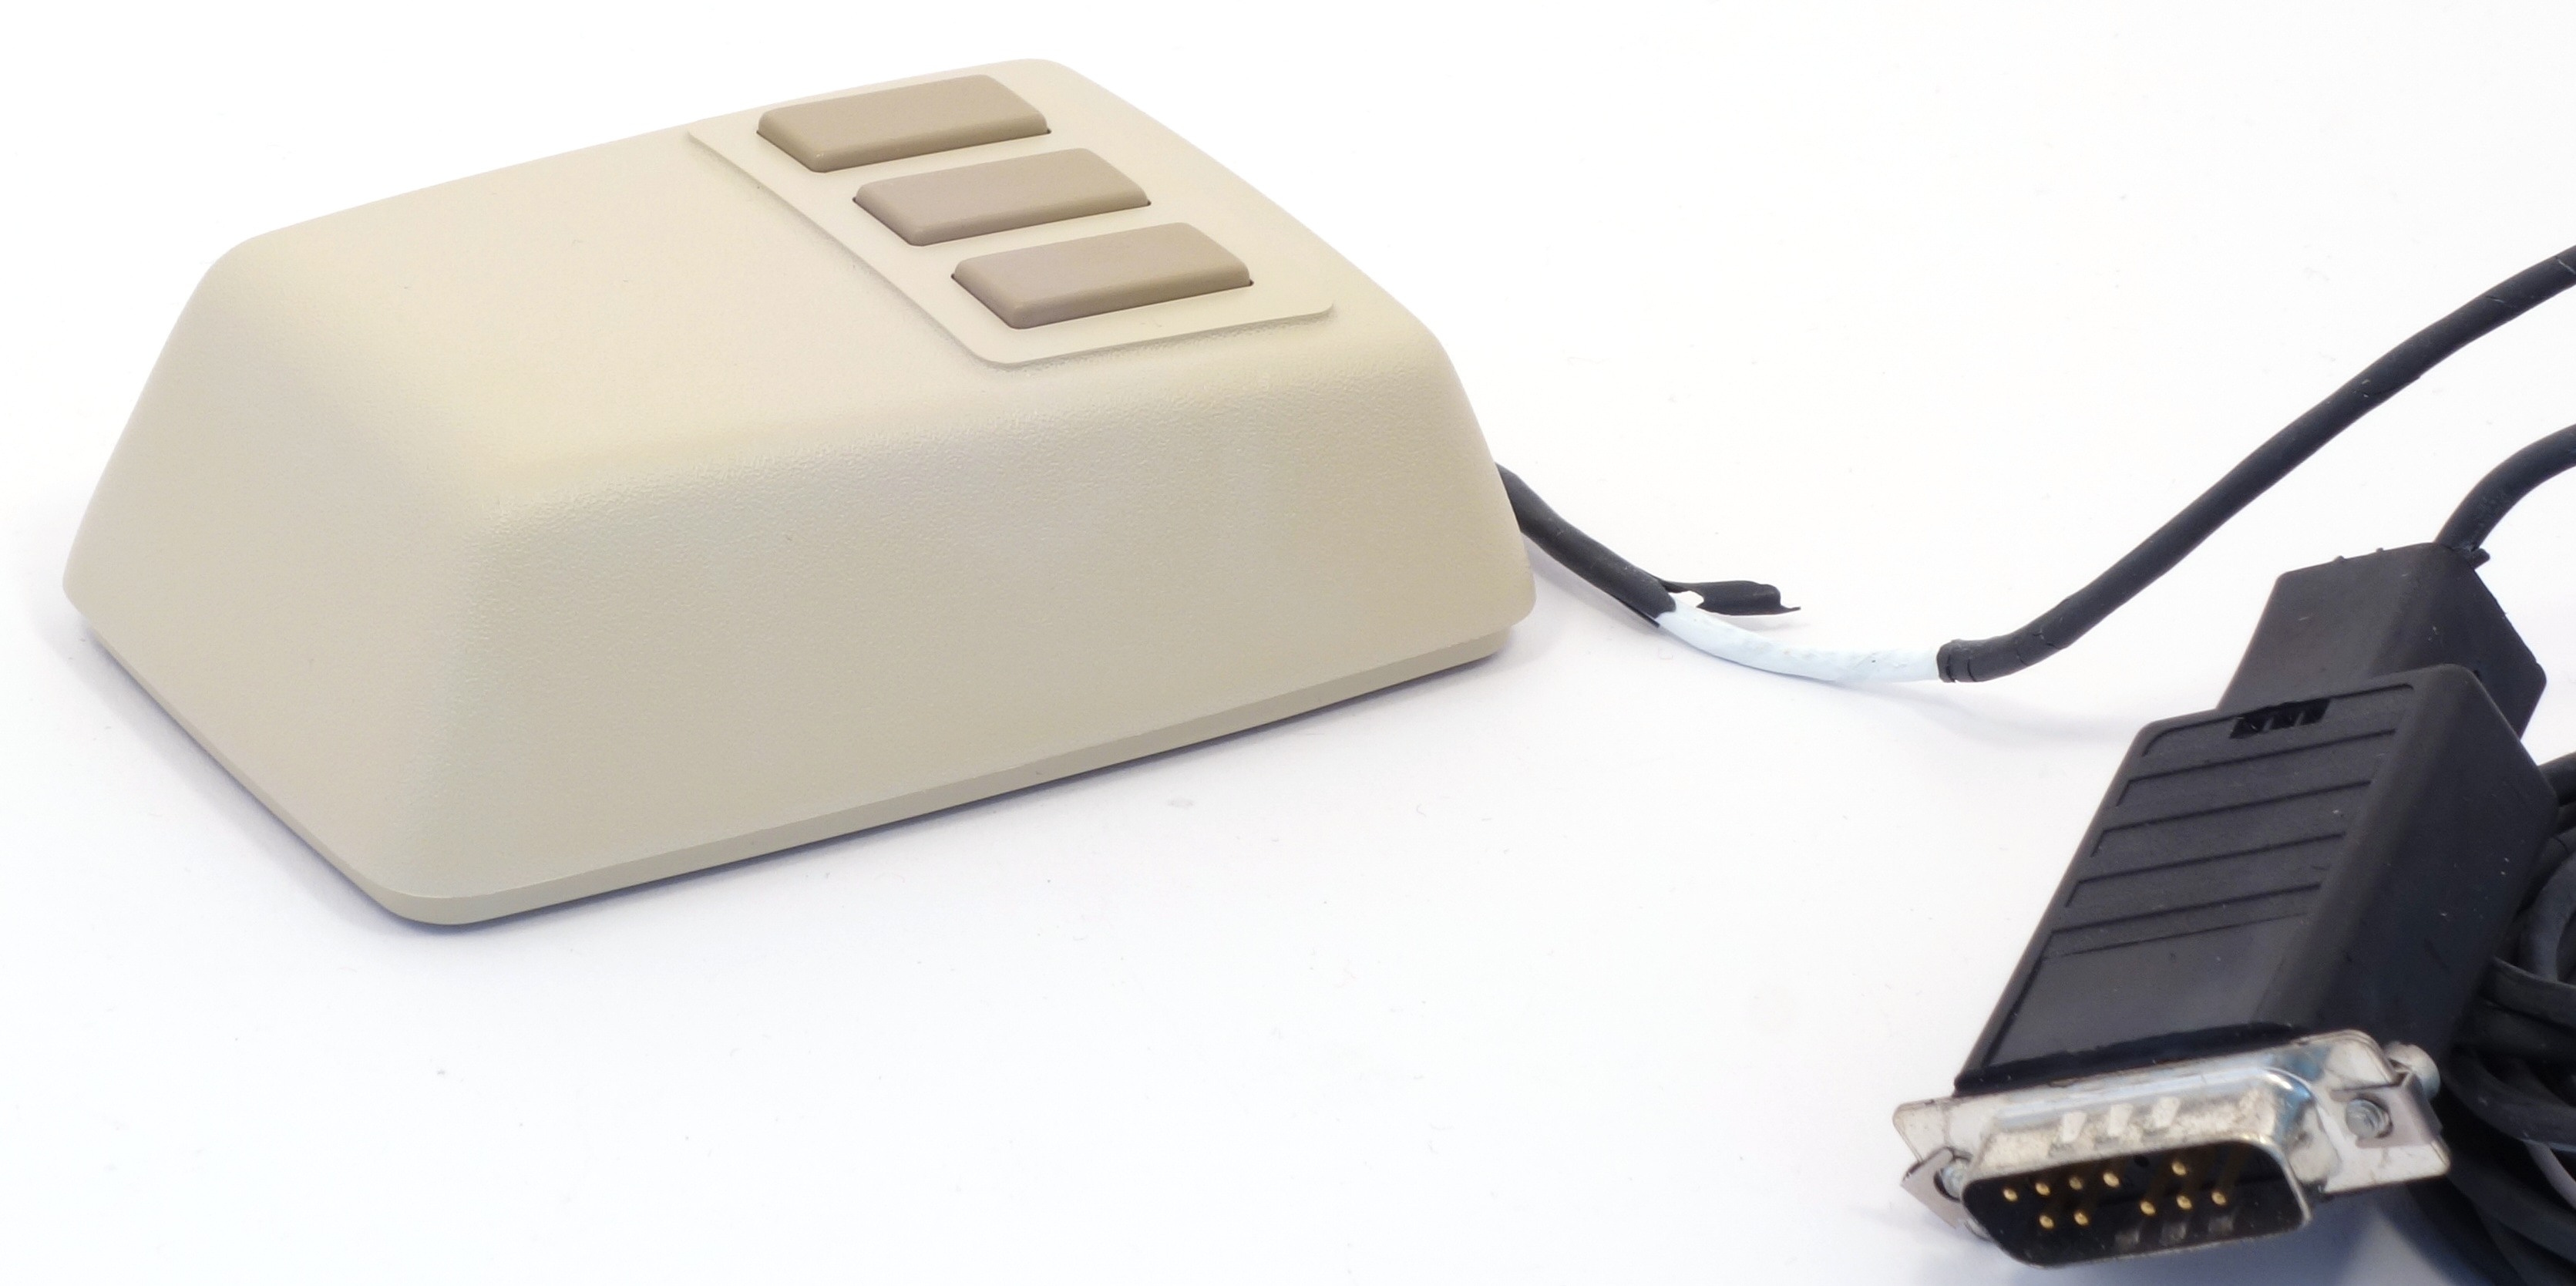
\includegraphics[scale=0.6]{1983_dec_vs10x_ea_mouse/pic_30.jpg}
    \caption{DEC VS10X-EA Mouse}
    \label{fig:DecVS10XPic}
\end{figure}

By contrast with the prototype mouse’s body (a parallelepiped with three rectangular buttons), the body of DEC VS10X-EA has a smoother shape with a substantially inclined sides and smooth transitions between the faces. Both mice have same internals, so the smoother shape is achieved at the cost of the increased size, and Hawley mouse’s rectangle is still easily seen on the bottom (fig. \ref{fig:DecVS10XTopAndBottom}). Obviously, such improvements had a positive effect on the ergonomics of the device.

\begin{figure}[h]
    \centering
    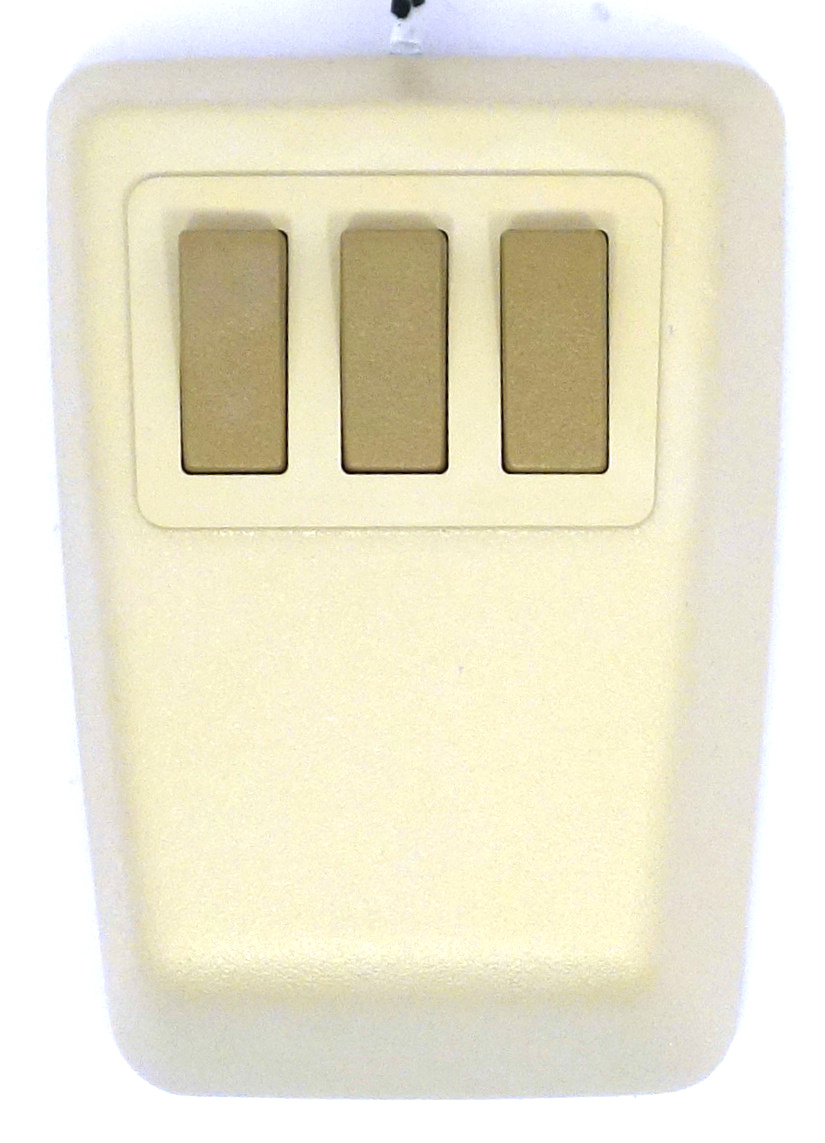
\includegraphics[scale=0.55]{1983_dec_vs10x_ea_mouse/top_60.jpg}
    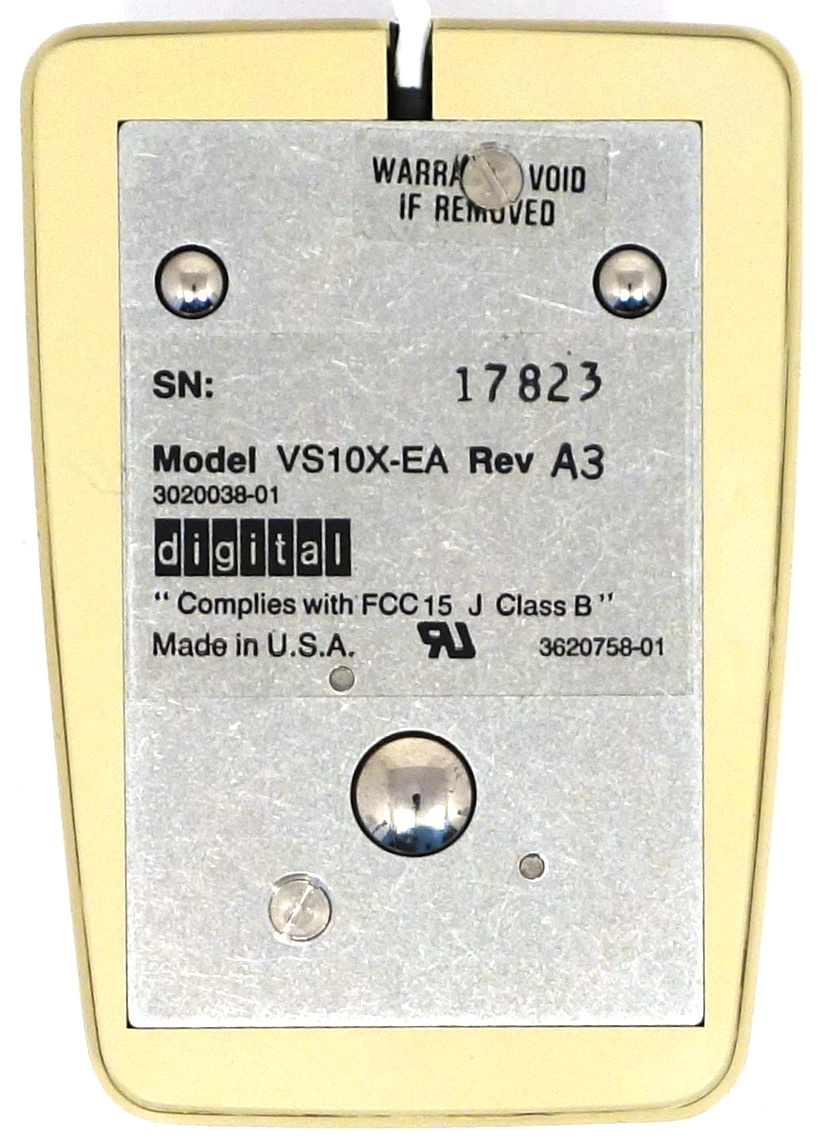
\includegraphics[scale=0.55]{1983_dec_vs10x_ea_mouse/bottom_30.jpg}
    \caption{DEC VS10X-EA Mouse, top and bottom views}
    \label{fig:DecVS10XTopAndBottom}
\end{figure}

The underside is made of metal (fig. \ref{fig:DecVS10XTopAndBottom}). The rotation is registered by a smooth steel ball in the center, while two smaller balls act as legs to minimize friction. The mouse was not supplied with a mouse pad, and  the VAXstation 100 user manual suggests to  put mouse on a plain sheet of paper \cite{manual}.

A removable ring that allows you to remove the ball to remove collected debris is not yet provided in this model, so complete disassembly is necessary for cleaning.

\begin{figure}[h]
    \centering
    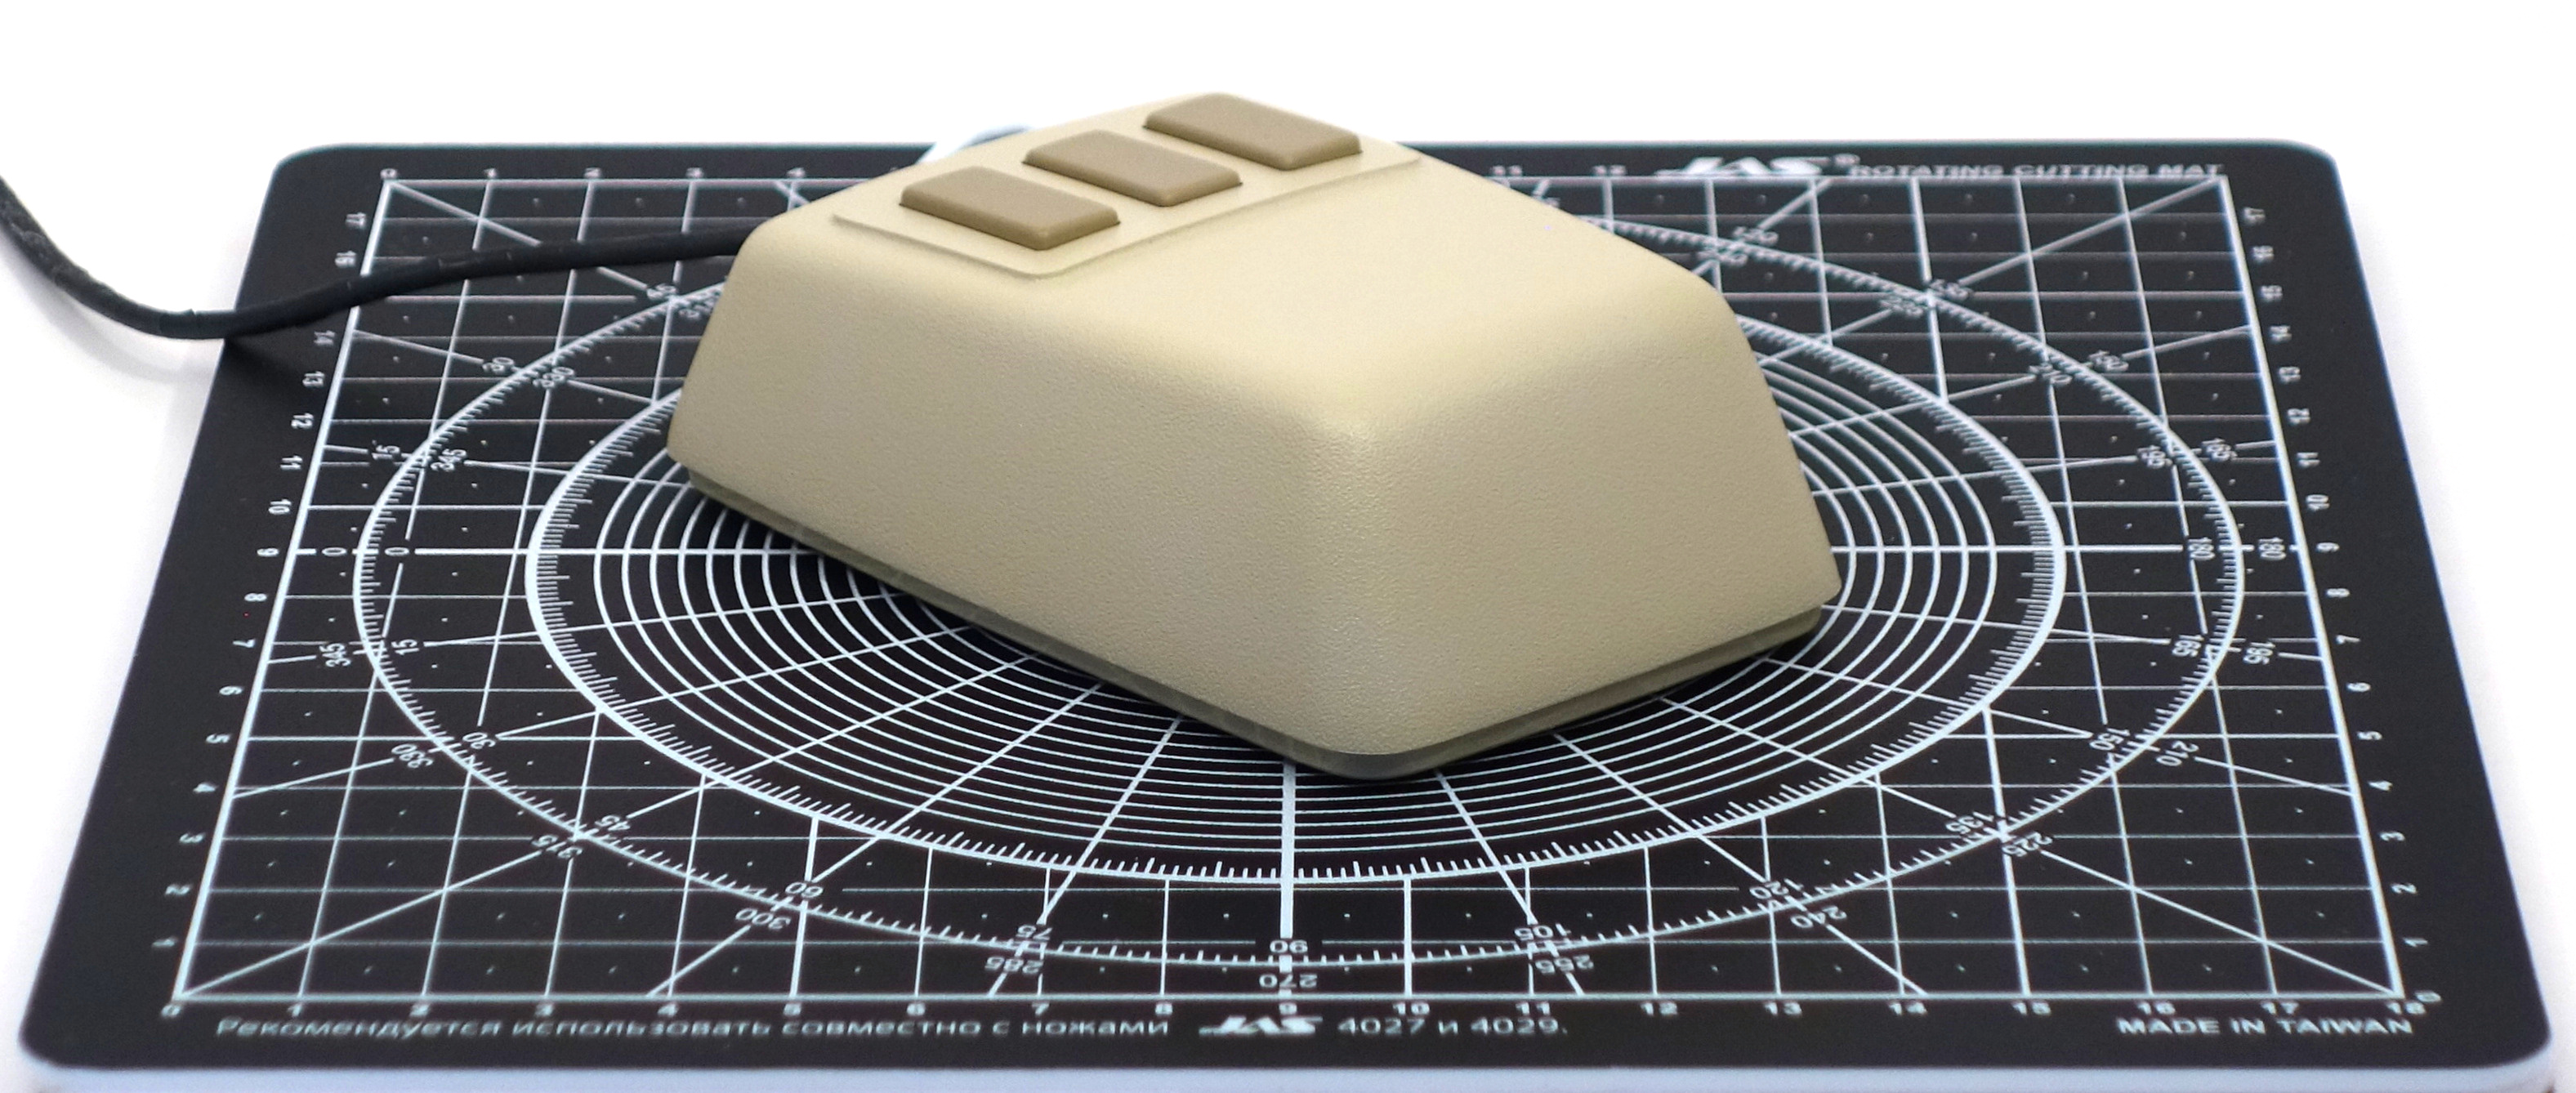
\includegraphics[scale=0.7]{1983_dec_vs10x_ea_mouse/size_30.jpg}
    \caption{DEC VS10X-EA on a graduated pad with a grid step of 1~cm}
    \label{fig:DecVS10XSize}
\end{figure}

The mouse has a small size, typical for mice of the 1980s (fig. \ref{fig:DecVS10XSize}), and so the hand can only lean on the body to a small extent (Fig. \ref{fig:DecVS10XHand}).
\begin{figure}[h]
    \centering
    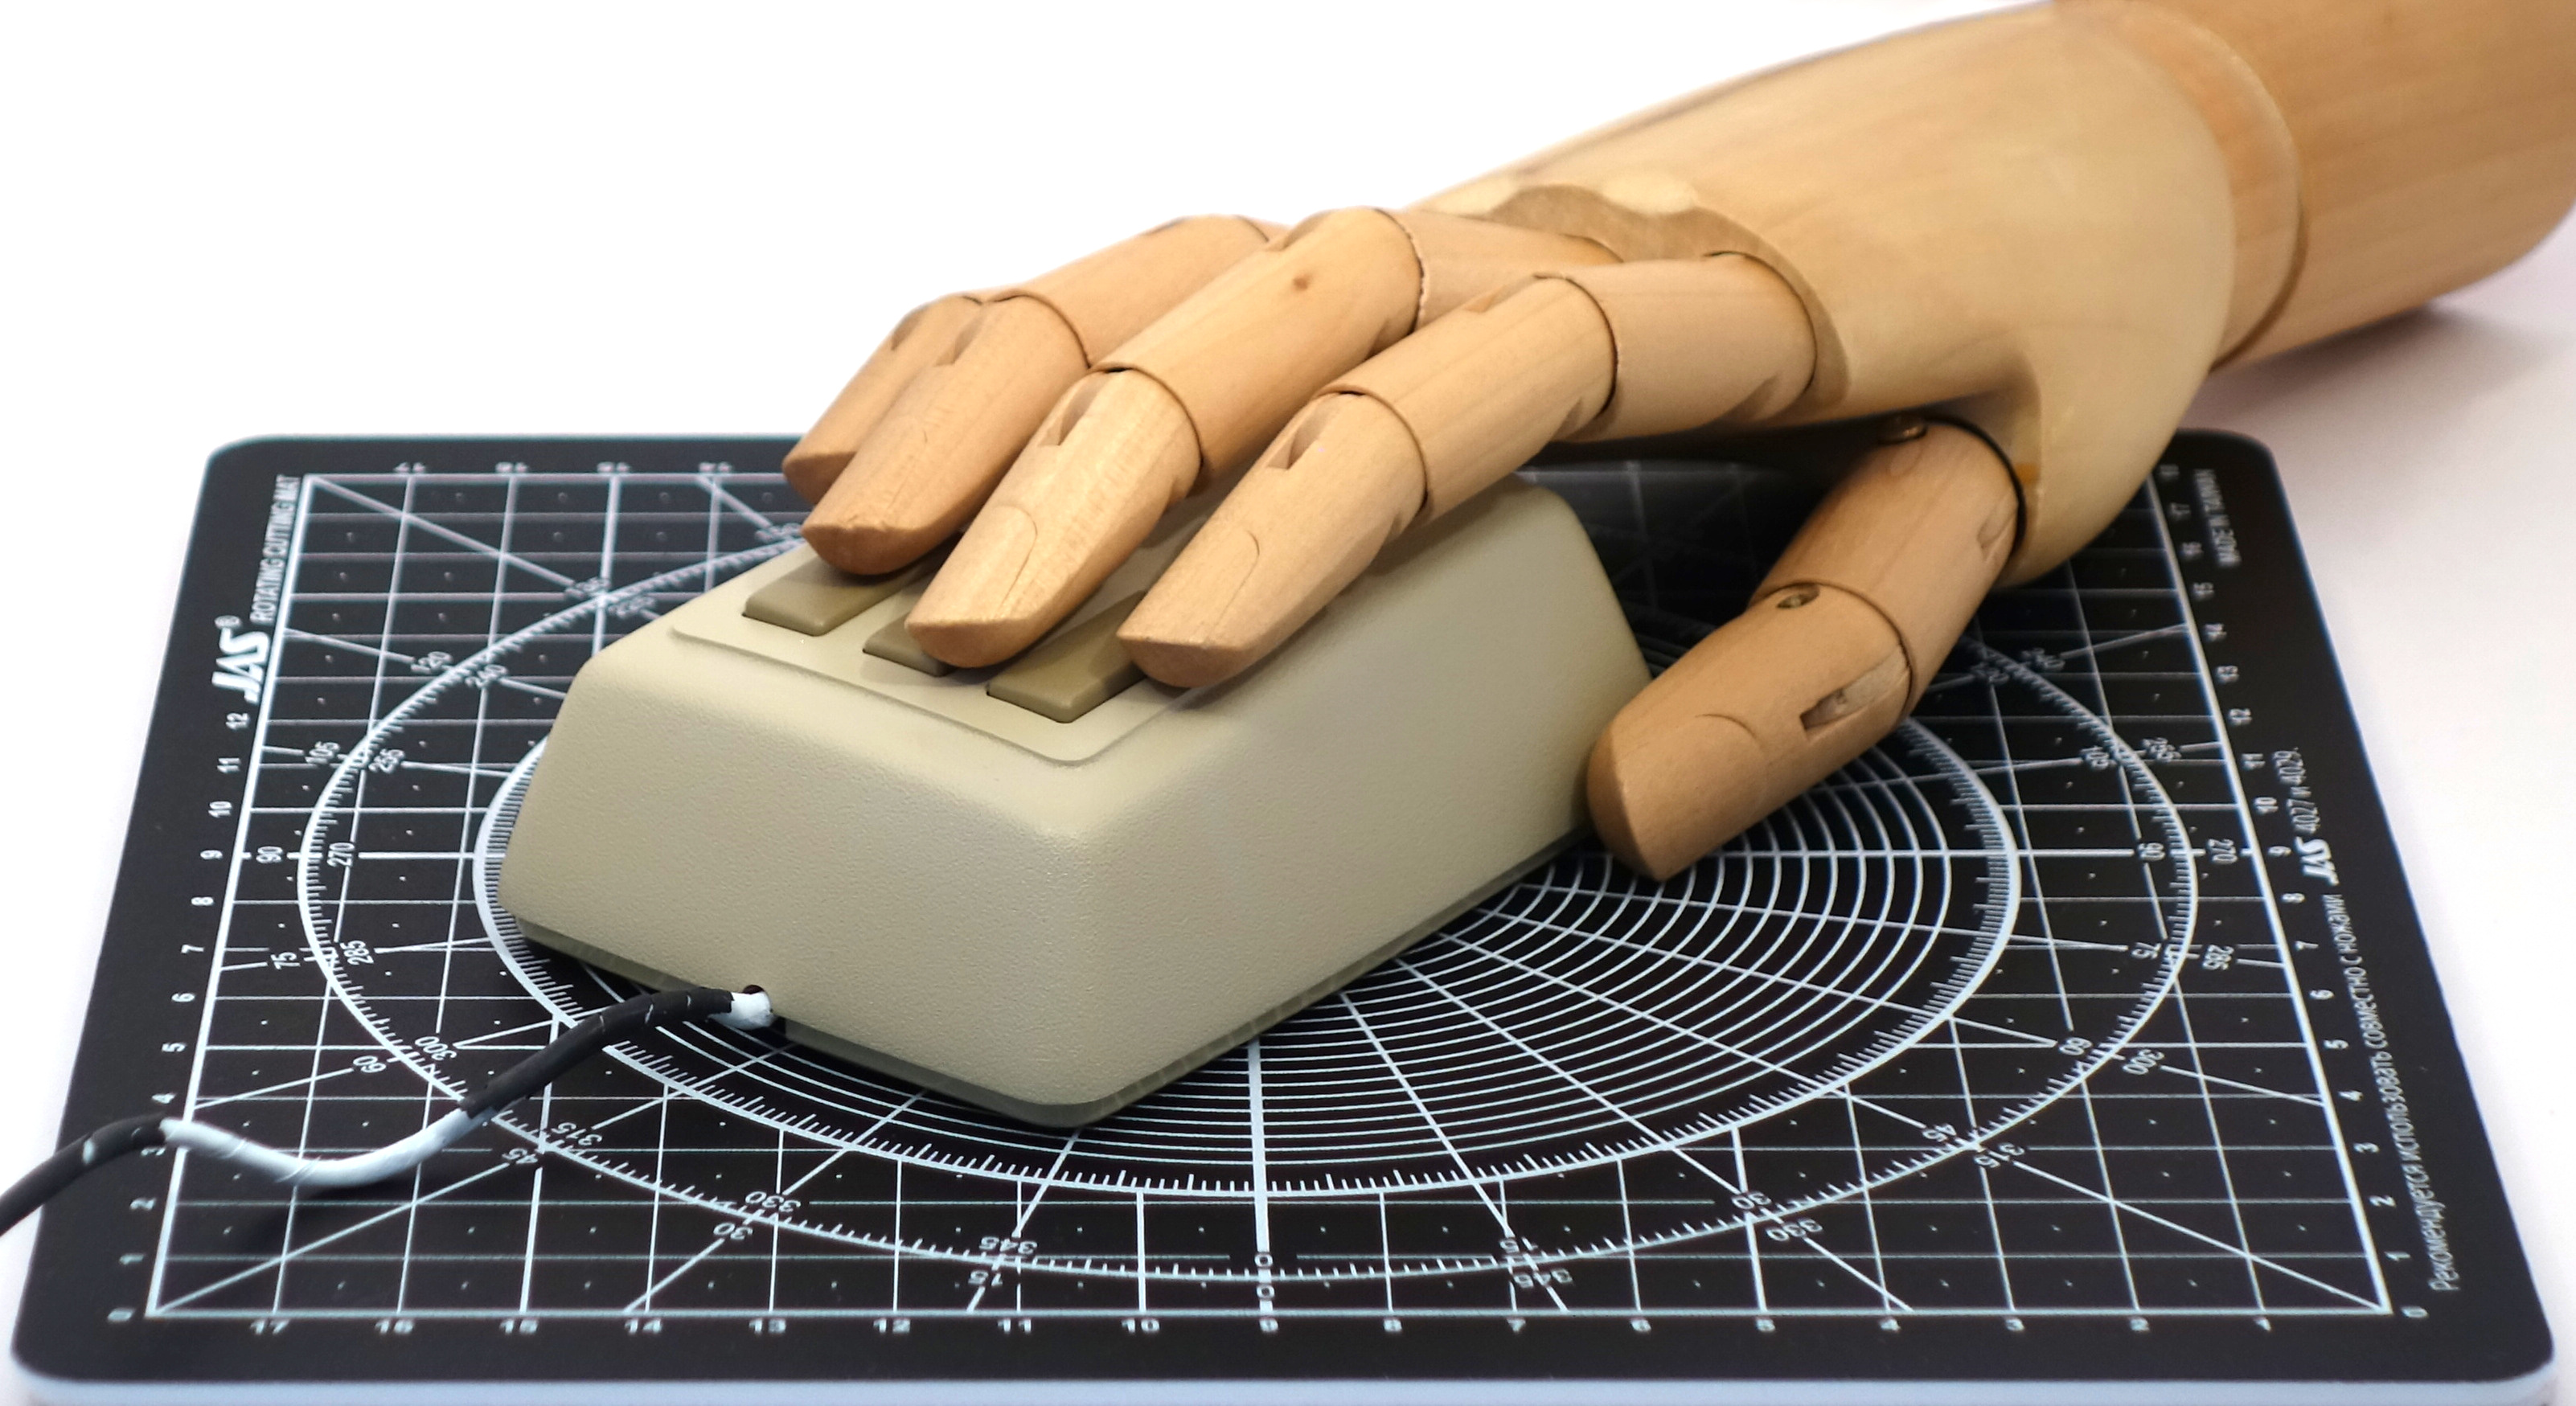
\includegraphics[scale=0.7]{1983_dec_vs10x_ea_mouse/hand_30.jpg}
    \caption{DEC VS10X-EAI with a human hand model}
    \label{fig:DecVS10XHand}
\end{figure}

Mouse internals are shown in figure \ref{fig:DecVS10XInside}. The removable solid protection of the ball is worthy of mention: it requires additional disassembly operations to remove garbage. In this mouse, contact encoders (with four contacts for greater reliability) are used, which are based on a metal contact drum instead of the more common disk in subsequent models.

~

\begin{figure}[h]
    \centering
    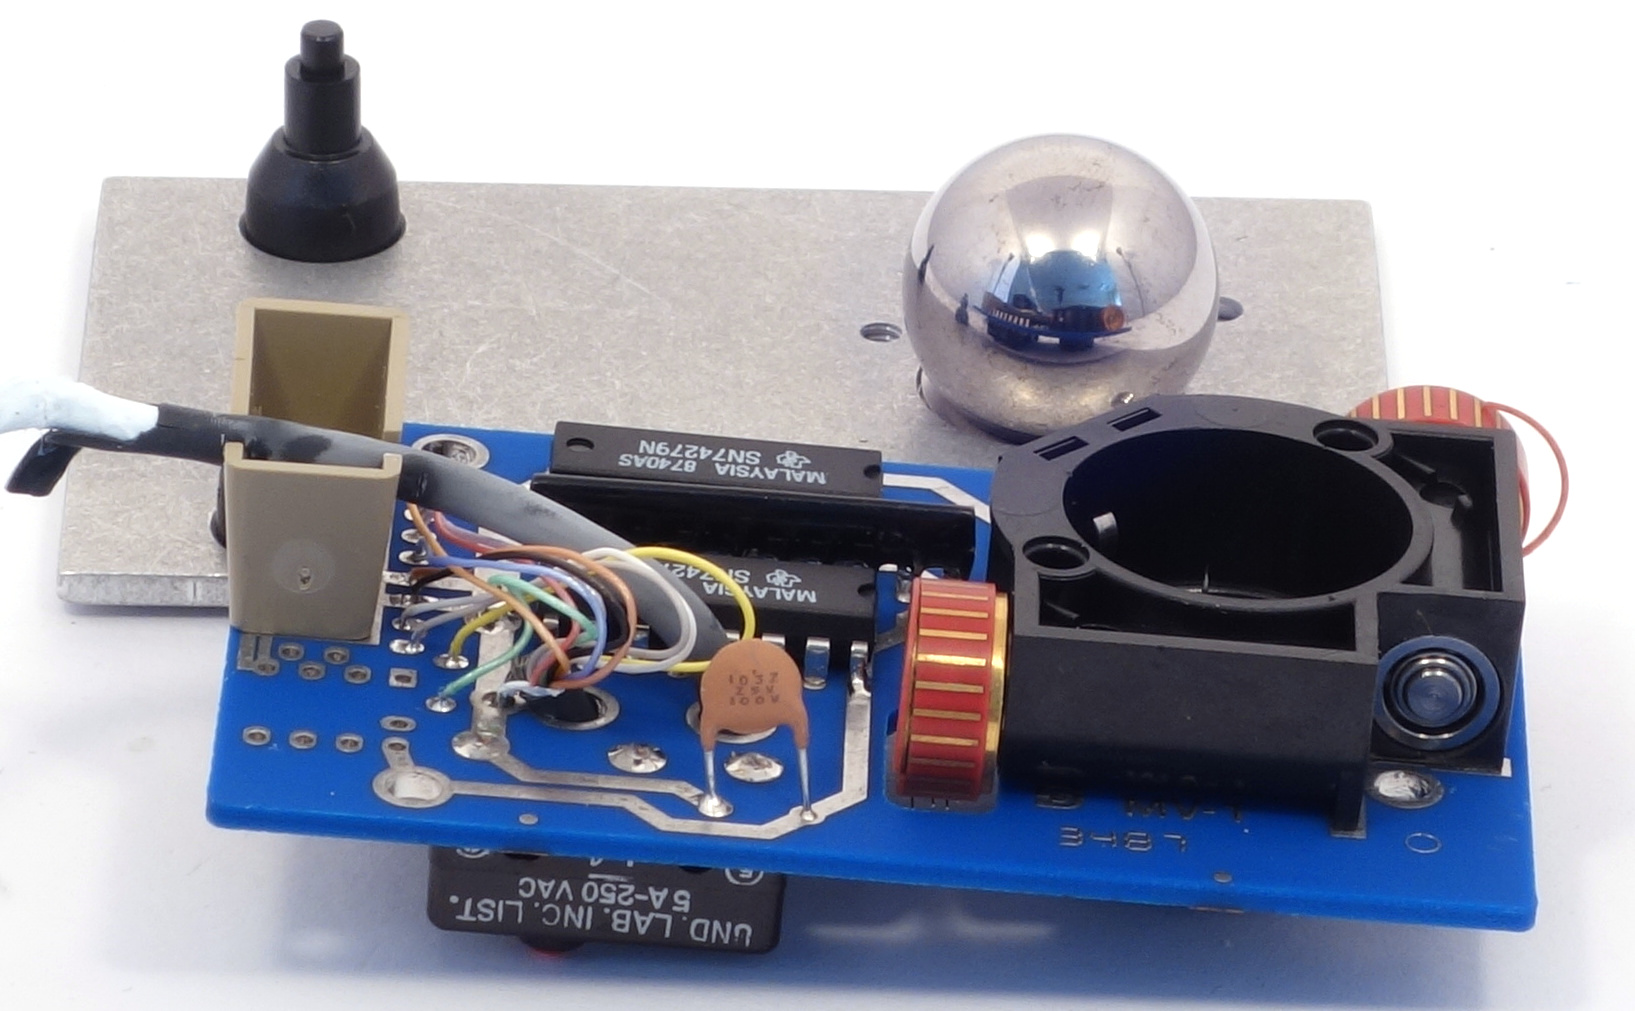
\includegraphics[scale=1]{1983_dec_vs10x_ea_mouse/inside_30.jpg}
    \caption{DEC VS10X-EA disassembled}
    \label{fig:DecVS10XInside}
\end{figure}

\begin{thebibliography}{9}
\bibitem{hawley} Hawley Mouse House \url{https://oldmouse.com/mouse/hawley/}

\bibitem{mouses} Hawley Mark II X063X Mouses \url{https://oldmouse.com/mouse/hawley/X063X.shtml}

\bibitem{pat} Transducer for a display-oriented pointing device \url{https://patents.google.com/patent/US3892963A/en}

\bibitem{reddit} Another DEC mouse \url{https://www.reddit.com/r/vintagecomputing/comments/mm4des/another_dec_mouse/}

\bibitem{manual} VAXstation 100 User Guide \url{http://www.bitsavers.org/pdf/dec/vax/vaxstation100/AA-N660A-TE_VAXstation_100_Users_Guide_Jun84.pdf}
\end{thebibliography}
\end{document}
